%----------------------------------------------------------------------------------------
%    PACKAGES AND OTHER DOCUMENT CONFIGURATIONS
%----------------------------------------------------------------------------------------
\documentclass[paper=a4, fontsize=13pt, twoside=semi]{scrartcl}
\usepackage[utf8]{inputenc}
\usepackage[catalan]{babel}
\usepackage[fixlanguage]{babelbib}
\selectbiblanguage{catalan}

\addtokomafont{sectioning}{\normalfont\scshape}
\usepackage[T1]{fontenc}
\usepackage{lmodern}
\usepackage{tocstyle}
\usetocstyle{standard}
\renewcommand*\descriptionlabel[1]{\hspace\labelsep\normalfont\bfseries{#1}}

\usepackage{fancyhdr}
\pagestyle{fancyplain}
\fancyhead[LO]{\thepage}
\fancyhead[CO]{}
\fancyhead[RO]{\nouppercase{\mytitle}}
\fancyhead[LE]{\nouppercase{\leftmark}}
\fancyhead[CE]{}
\fancyhead[RE]{\thepage}
\fancyfoot{}
\renewcommand{\headrulewidth}{0.3pt}
\renewcommand{\footrulewidth}{0pt}
\setlength{\headheight}{13.6pt}

\usepackage{etoolbox}
\pretocmd{\section}{\cleardoubleevenemptypage}{}{}
\pretocmd{\part}{\cleardoubleevenemptypage\thispagestyle{empty}}{}{}

\renewcommand\partheadstartvskip{\clearpage\null\vfil} 
\renewcommand\partheadmidvskip{\par\nobreak\vskip 20pt\thispagestyle{empty}}

\setlength{\parindent}{0pt}
\setlength{\parskip}{0.3\baselineskip plus2pt minus2pt}
\newcommand{\sk}{\medskip\noindent}

\usepackage{hyperref}
\hypersetup{colorlinks, citecolor=black, filecolor=black, linkcolor=black, urlcolor=black}

%----------------------------------------------------------------------------------------
%    MATHS AND ENVIRONMENTS
%----------------------------------------------------------------------------------------
\usepackage{amsmath,amsfonts,amsthm,amssymb}
\usepackage{xfrac}
\usepackage[a]{esvect}
\usepackage{pgfplots}
\usepackage{tikz}
\usepackage{thmtools}
\usepackage{environ}

\usepackage{siunitx}

\newcommand*{\dif}{\mathrm{d}}
\newcommand*{\diff}{\mathop{}\!\mathrm{d}}
\newcommand*{\vnabla}{\vec{\nabla}}

\numberwithin{equation}{section}
\numberwithin{figure}{section}
\numberwithin{table}{section}

\usepackage{enumerate}
\usepackage{booktabs}
\usepackage{float}
    % \setlength{\intextsep}{8pt}

\makeatletter
\renewcommand*\env@matrix[1][*\c@MaxMatrixCols c]{%
    \let\@ifnextchar\new@ifnextchar
    \array{#1}}
\makeatother

\usepackage{ccicons}
\usepackage{lipsum}

\makeatletter
\newcommand*\NoIndentAfterEnv[1]{%
  \AfterEndEnvironment{#1}{\par\@afterindentfalse\@afterheading}}
\makeatother
%\NoIndentAfterEnv{thm}
\NoIndentAfterEnv{defi}
\NoIndentAfterEnv{example}
\NoIndentAfterEnv{table}

%----------------------------------------------------------------------------------------
%    THEOREMS
%----------------------------------------------------------------------------------------
\makeatletter
\providecommand{\@fourthoffour}[4]{#4}  
\newcommand\fixstatement[2][\proofname\space del]{%
    \ifcsname thmt@original@#2\endcsname
        \AtEndEnvironment{#2}{%
            \xdef\pat@label{\expandafter\expandafter\expandafter
                \@fourthoffour\csname thmt@original@#2\endcsname\space\@currentlabel}%
            \xdef\pat@proofof{\@nameuse{pat@proofof@#2}}%
        }%
    \else
        \AtEndEnvironment{#2}{%
            \xdef\pat@label{\expandafter\expandafter\expandafter
                \@fourthoffour\csname #1\endcsname\space\@currentlabel}%
            \xdef\pat@proofof{\@nameuse{pat@proofof@#2}}%
        }%
    \fi
    \@namedef{pat@proofof@#2}{#1}%
}
\globtoksblk\prooftoks{1000}
\newcounter{proofcount}
\NewEnviron{proofatend}{%
    \edef\next{%
        \noexpand\begin{proof}[\pat@proofof\space\pat@label]%
        \unexpanded\expandafter{\BODY}}%
    \global\toks\numexpr\prooftoks+\value{proofcount}\relax=\expandafter{\next\end{proof}}
    \stepcounter{proofcount}}
\def\printproofs{%
      \count@=\z@
      \loop
        \the\toks\numexpr\prooftoks+\count@\relax
           \ifnum\count@<\value{proofcount}%
           \advance\count@\@ne
      \repeat}
\makeatother

\declaretheorem[style=plain,name=Teorema,qed=$\square$,numberwithin=section]{thm}
\declaretheorem[style=plain,name=Corol·lari,qed=$\square$,sibling=thm]{cor}
\declaretheorem[style=plain,name=Lemma,qed=$\square$,sibling=thm]{lem}
    \fixstatement{thm}
    \fixstatement[Demostració del]{lem}

\declaretheorem[style=definition,name=Definició,qed=$\blacksquare$,numberwithin=section]{defi}
\declaretheorem[style=definition,name=Exemple,qed=$\blacktriangle$,numberwithin=section]{example}

%----------------------------------------------------------------------------------------
%    PDF INFO
%----------------------------------------------------------------------------------------
\newcommand*{\mytitle}{Ones i òptica}
\newcommand*{\myauthor}{Alfredo Hernández Cavieres} 
\newcommand*{\myuni}{Universitat Autònoma de Barcelona, Departament de Física}
\newcommand*{\mydate}{\normalsize 2012-2013}

\usepackage{hyperxmp}
\hypersetup{pdfauthor={\myauthor}, pdftitle={\mytitle}}

%----------------------------------------------------------------------------------------
%    TITLE SECTION AND DOCUMENT BEGINNING
%----------------------------------------------------------------------------------------
\newcommand{\horrule}[1]{\rule{\linewidth}{#1}}
\title{
    \normalfont
    \small \scshape{\myuni} \\ [25pt] 
    \horrule{0.5pt} \\[0.4cm]
    \huge \mytitle \\
    \horrule{2pt} \\[0.5cm]
}
\author{\myauthor}
\date{\mydate}

\begin{document}

\clearpage\maketitle
\thispagestyle{empty}
\addtocounter{page}{-1}

%----------------------------------------------------------------------------------------
%    LLICÈNCIA
%----------------------------------------------------------------------------------------
\section*{}\thispagestyle{empty}
\begin{centering}
    \huge \ccbyncsaeu
    
    \normalsize Aquesta obra està subjecta a una llicència de 
    
    Reconeixement-NoComercial-CompartirIgual 4.0 
    
    Internacional de Creative Commons.
    
\end{centering}

%----------------------------------------------------------------------------------------
%    TABLE OF CONTENTS
%----------------------------------------------------------------------------------------
\tableofcontents

%----------------------------------------------------------------------------------------
%    SECTIONS
%----------------------------------------------------------------------------------------
\part*{Ones}
\addcontentsline{toc}{part}{Ones}
    %----------------------------------------------------------------------------------------
%    OSCIL·LACIONS
%----------------------------------------------------------------------------------------
\section{Oscil·lacions}
\subsection{Moviment oscil·latori harmònic simple}

\subsubsection*{Equació del moviment}
\begin{align}
    \boxed{\frac{\partial^{2} x}{\partial t^{2}} = - \frac{k}{m} x}
\end{align}

\subsubsection*{Correlació amb MCU}
%----------------------------------------------------------------------------------------
\subsection{Energia d'un oscil·lador}
\subsubsection*{Energia potencial ($U$)}
\begin{align}
    \boxed{U = \frac{1}{2} k x^{2} = \frac{1}{2} k A^{2} \cos^{2} (\omega t + \varphi_{0})}
\end{align}

\subsubsection*{Energia cinètica ($K$)}
\begin{align}
    \boxed{K = \frac{1}{2} m v^{2} = \frac{1}{2} k A^{2} \sin^{2} (\omega t + \varphi_{0})}
\end{align}

\subsubsection*{Energia mecànica total ($E$)}
\begin{align}
    \boxed{E = U + K = \frac{1}{2} k A^{2}}
\end{align}
\begin{figure}[H]
\centering
    WIP: GRAFIC BONIC 
\caption{Pou de potencial. La particula està confinada en $x \in [-A, +A]$}
\end{figure}
%----------------------------------------------------------------------------------------
\subsection{Pèndol simple}
\begin{figure}[H]
\centering
    WIP: GRAFIC BONIC 
\caption{Pèndol simple}
\end{figure}

\subsubsection*{Equació del moviment}
\begin{align}
    \boxed{\frac{\partial^{2} \phi}{\partial t^{2}} = - \frac{g}{L} \sin \phi}
\end{align}

%----------------------------------------------------------------------------------------
\subsection{Pèndol físic}
\begin{figure}[H]
\centering
    WIP: GRAFIC BONIC 
\caption{Pèndol físic}
\end{figure}

\subsubsection*{Equació del moviment}
\begin{align}
    \boxed{\frac{\partial^{2} \phi}{\partial t^{2}} = - \frac{M g L}{I} \sin \phi}
\end{align}

%----------------------------------------------------------------------------------------
\subsection{Pèndol de torsió}
\begin{figure}[H]
\centering
    WIP: GRAFIC BONIC 
\caption{Pèndol de torsió}
\end{figure}

\subsubsection*{Equació del moviment}
\begin{align}
    \boxed{\frac{\partial^{2} \phi}{\partial t^{2}} = - \frac{k \phi}{I}}
\end{align}

%----------------------------------------------------------------------------------------
\subsection{Oscil·lacions amortides}

\subsubsection*{Equació del moviment}
\begin{align}
    \boxed{\frac{\partial^{2} x}{\partial t^{2}} + \frac{\gamma}{m} \frac{\partial x}{\partial t} + \frac{k}{m} x = 0}
\end{align}

\subsubsection*{Subamortiment}

\subsubsection*{Amortiment crític i sobreamortiment}
\begin{figure}[H]
\centering
    WIP: GRAFIC BONIC 
\caption{Posició ($x$) d'un oscil·lador en amortiment crític ($\beta \ll \omega_{0}$) i sobreamortiment ($\beta \gg \omega_{0}$). Per a l'amortiment crític, $t$ per a l'equilibri és el mínim possible}
\end{figure}

\subsubsection*{Energia}
\begin{align}
    \boxed{E = \frac{1}{2} k A^{2} = \frac{1}{2} m \omega_{0}^{2} A_{0}^{2} e^{-2 \beta t}}
\end{align}
\begin{figure}[H]
\centering
    WIP: GRAFIC BONIC 
\caption{Amortiment de l'energia d'un oscil·lador. Notem que podem definir un temps d'amortiment de l'energia $\tau_{0}' = \frac{m}{\gamma}$, tal que l'energia sigui $E(\tau_{0}') = E_{max}/e$. }
\end{figure}

%----------------------------------------------------------------------------------------
\subsection{Oscil·lacions forçades}

\subsubsection*{Equació del moviment}
\begin{align}
    \boxed{m \frac{\partial^{2} x}{\partial t^{2}} + \gamma \frac{\partial x}{\partial t} + m \omega_{0}^{2} x = F_{0} \cos (\omega t)}
\end{align}
    %----------------------------------------------------------------------------------------
%    ONES
%----------------------------------------------------------------------------------------
\section{Ones}
\begin{itemize}
    \item Moviment ondulatori: transporta $\begin{cases} E \text{ (energia)} \\ \vec{P} \text{ (moment lineal)} \\ \vec{L} \text{ (moment angular)} \end{cases}$
    \item Tipus:
        \subitem Mecàniques: requereixen medi.
        \subitem Electromagnètiques: no requereixen medi.
\end{itemize}

\subsection{Característiques}
\begin{itemize}
    \item Focus emissor: origen de la pertorbació. Aporta energia.
    \item Material: les forces intermoleculars són les responsables de la propagació de l'ona: $v_{p} \propto F_{\text{int}}$; en ones electromagnètiques, $v_{p} = c$.
    \item Tipus d'ones:
        \subitem Transversals: la pertorbació és perpendicular a $v_{p}$.
        \subitem Longitudinals: la pertorbació és paral·lela a $v_{p}$.
    \item Front d'ona:
        \subitem Ona esfèrica:
        \subitem Ona plana:
    \item Magnituds:
        \subitem Velocitat de propagació: no depèn del focus i és $\perp$ als fronts d'ona. $\boxed{v_{p} = \frac{\partial x}{\partial t}}$, $\boxed{v = \lambda \nu}$.
        \subitem Freqüència: $\boxed{\nu = \frac{1}{T}}$.
        \subitem Freqüència angular: $\boxed{\omega = 2 \pi \nu}$.
        \subitem Nombre d'ones: $\boxed{k = \frac{2 \pi}{\lambda}}$.
\end{itemize}

%----------------------------------------------------------------------------------------
\subsection{Equació d'ona}
La velocitat de propagació d'una ona en una corda oscil·lant és:
\begin{align}
    \boxed{v_{p} = \sqrt{\frac{T}{\mu}}}
\end{align}
on $T \equiv$ tensió de la corda i $\mu \equiv$ densitat lineal de la corda.
\begin{align}
    \boxed{\frac{\partial^{2} y}{\partial t^{2}} = v_{p}^{2} \frac{\partial^{2} y}{\partial x^{2}}}
\end{align}

%----------------------------------------------------------------------------------------
\subsection{Ones viatgeres}
Compleixen l'equaciçó d'ones aquelles ones tal que:
\begin{align}
    \boxed{f(x,t) = f(x \mp v t)}
\end{align}
\begin{figure}[H]
\centering
    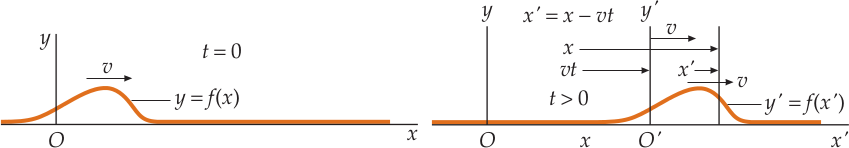
\includegraphics[width=\textwidth]{images/2/23-viatgeres.png}
\caption{Pols de corda en moviment. Es compleix que $x' = x - vt$}
\end{figure}

%----------------------------------------------------------------------------------------
\subsection{Ones harmòniques}
\begin{align}
    \boxed{\psi (x,t) = \psi_{0} \sin (x \mp v t)}
\end{align}
\begin{align}
    \boxed{y (x,t) = A \sin (kx - \omega t)}
\end{align}
\begin{figure}[H]
\centering
   %\def\svgwidth{\columnwidth}\input{./images/2/2-2-harmoniques.pdf_tex} 
   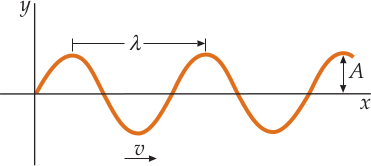
\includegraphics[width=0.5\textwidth]{images/2/24-harmonica.png}
\caption{Representació gràfica d'una ona harmònica en funció de $x$. Es compleix que $\lambda = v T$}
\end{figure}

\subsubsection*{Energia (en una corda)}
\begin{align}
    \boxed{\Delta E = \frac{1}{2} k_{m} A^{2}} \qquad \text{on } k_{m} = m \omega^{2}
\end{align}
\begin{align}
    \Delta E = \frac{1}{2} \mu v \Delta t \omega^{2} A^{2} \Rightarrow \boxed{P_{m} = \frac{1}{2} \mu v \omega^{2} A^{2}}
\end{align}
\subsubsection*{Diferència de fase}
Sigui $\psi (x,t) = \psi_{0} \sin (\omega t \pm kx \varphi_{0})$. Llavors definim la diferència de fase com:
\begin{align}
    \boxed{\Delta \varphi = \varphi_{2} - \varphi_{1}}
\end{align}
\begin{itemize}
    \item Per a temps $t$ fix:
        $\begin{gathered} \boxed{\Delta \varphi = k \Delta x = \frac{2 \pi}{\lambda} \Delta x}. \end{gathered}$
    \item Per a posició $x$ fixa:
        $\begin{gathered} \boxed{\Delta \varphi = \omega \Delta t \ = 2 \pi \nu \Delta t}. \end{gathered}$
\end{itemize}
Quan tenim dues ones harmòniques, $\forall m \in \mathbb{N}$, les dues ones estaran:
\begin{itemize}
    \item En fase: $\boxed{\Delta \varphi = 0 \pm 2 \pi m}$.
    \item En contrafase: $\boxed{\Delta \varphi = (2m \pm 1) m}$.
    \item En quadratura: $\boxed{\Delta \varphi = (\frac{1}{2} + m) \pi}$.
\end{itemize}

%----------------------------------------------------------------------------------------
\subsection{Principi de superposició lineal}

%----------------------------------------------------------------------------------------
\subsection{Interferències}
\subsubsection*{Ones estacionàries}
\subsubsection*{Ones harmòniques}
\subsubsection*{Polsació d'ones}
\subsubsection*{Patrons d'inteferència}
\begin{figure}[H]
\centering
    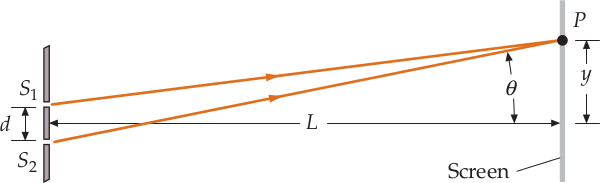
\includegraphics[width=0.8\textwidth]{images/2/26-doble-escletxa.png}
\caption{Diagrama de patró d'inteferències de doble escletxa a una paret. Les distàncies entre elles són $y_{n}$, on $n$ és l'ordre d'interferència}
\end{figure}
\begin{align}
    \boxed{y_{n} = \frac{x \lambda}{d} n}
\end{align}
\subsubsection*{Diferents eixos de vibració}
\begin{figure}[H]
\centering
    WIP: GRAFIC BONIC 
\caption{Figures de Lisajous, la resultant de la superposició és una ona polaritzada}
\end{figure}
\subsubsection*{Difracció}
\begin{figure}[H]
\centering
    WIP: GRAFIC BONIC 
\caption{Difracció d'una ona en una escletxa}
\end{figure}
%----------------------------------------------------------------------------------------
\subsection{Intensitat}
\begin{align}
    \boxed{I = \frac{\Delta E}{\Delta S \Delta t}} \quad \left[ \si{\W\per\m\squared} \right]
\end{align}

\subsubsection*{Mesura de la intensitat}
El rang de $I$ audibles pels humans és $\begin{cases} I_{max} = \SI{1}{\W\per\m\squared} \\ I_{min} = \SI{10 e-12}{\W\per\m\squared} \equiv I_{0} \end{cases}$

Així doncs, definim el nivell d'intensitat com:
\begin{align}
    \boxed{\beta = 10 \log \left( \frac{I}{I_{0}} \right)} \quad [\si{\dB}]
\end{align}

\subsubsection*{Atenuació per propagació}
\begin{itemize}
    \item Circulars: $\begin{gathered} \boxed{I(r) = \frac{I_{0}}{2 \pi r}} \end{gathered}$.
    \item Esfèriques: $\begin{gathered} \boxed{I(r) = \frac{I_{0}}{4 \pi r^{2}}} \end{gathered}$.
\end{itemize}

\subsubsection*{Intensitat en dues dimensions}
\begin{align}
    \boxed{I = \frac{1}{2} \mu v \omega^{2} \frac{A^{2}}{\Delta S}}
\end{align}

\subsubsection*{Intensitat en tres dimensions}
\begin{align}
    I = \frac{1}{2} \rho \omega^{2} s_{0}^{2} v; \quad s_{0} = \frac{p_{0}}{\rho \omega v} \Rightarrow \boxed{I = \frac{1}{2} \frac{p_{0}^{2}}{\rho v}}
\end{align}

%----------------------------------------------------------------------------------------
\subsection{Efecte Doppler}
\begin{figure}[H]
\centering
    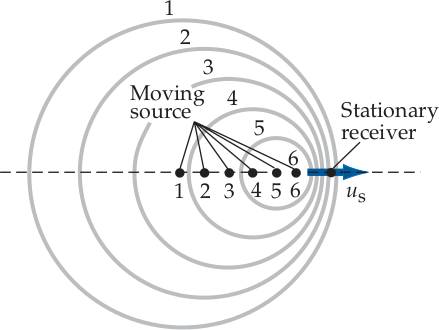
\includegraphics[width=0.5\textwidth]{images/2/28-doppler.png}
\caption{Diagrama de l'efecte Doppler per a un emisor $E$ i un receptor $R$ amb una velocitat relativa entre l'un respecte l'altre}
\end{figure}
\begin{align}
    \boxed{\nu_{r} = \frac{v_{p} \pm u_{r}}{v_{p} \mp u_{e}} \nu_{e}}
\end{align}

\subsubsection*{Criteri de signes}
\begin{itemize}
    \item $\begin{gathered} \frac{+}{-} \end{gathered}$: aproximació E-R $\Rightarrow \nu_{r} > \nu_{e}$.
    \item $\begin{gathered} \frac{-}{+} \end{gathered}$: allunyament E-R $\Rightarrow \nu_{r} < \nu_{e}$.
\end{itemize}
Observació: el medi trenca la simetria: $E \to R \neq R \to E$.
\subsubsection*{Ones de xoc}
\begin{figure}[H]
\centering
    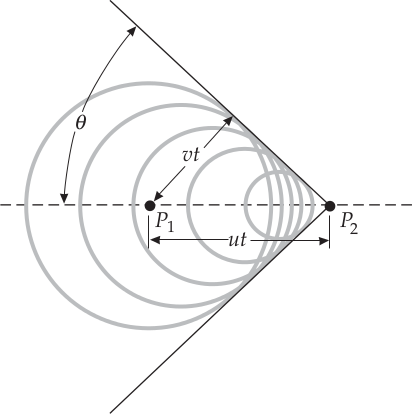
\includegraphics[width=0.5\textwidth]{images/2/28-ones-xoc.png}
\caption{Situació en què es produeixen ones de xoc}
\end{figure}
\begin{align}
    \boxed{\sin \theta = \frac{v}{u} = \text{(Nre. Mach)}^{-1}}
\end{align}

\subsubsection*{Efecte Doppler relativista}
\begin{align}
    \boxed{\nu_{r} = \nu_{e} \sqrt{\frac{1 \pm \beta}{1 \mp \beta}}} \qquad \text{on } \beta = \frac{v_{rel}}{c}
\end{align}
Té el mateix criteri de signes.
%----------------------------------------------------------------------------------------
\subsection{Propagació del so}
\begin{itemize}
    \item Líquids i sòlids: $\begin{gathered} v_{\text{so}} = \sqrt{\frac{B}{\rho}} \end{gathered}$.
    \item Gasos: $\begin{gathered} v_{\text{so}} = \sqrt{\frac{\gamma RT}{M}} \end{gathered}$.
\end{itemize}


\part*{Òptica}
\addcontentsline{toc}{part}{Òptica}
    %----------------------------------------------------------------------------------------
%    LA LLUM
%----------------------------------------------------------------------------------------
\section{La llum}
\subsection{Propietats de la llum}
\subsubsection*{Velocitat de la llum}
Els primers científics en intentar mesurar la velocitat de la llum han estat: Galileo Galilei (1638), Hippolyte Fizeau (1849), Michel Foucault (1850) i Albert Michelson (1880).
\begin{align}
    \boxed{c \equiv \SI{299792458}{\m\per\s}} \text{ (exactament)}.
\end{align}

\subsubsection*{Espectre electromagnètic}
\begin{figure}[H]
\centering
    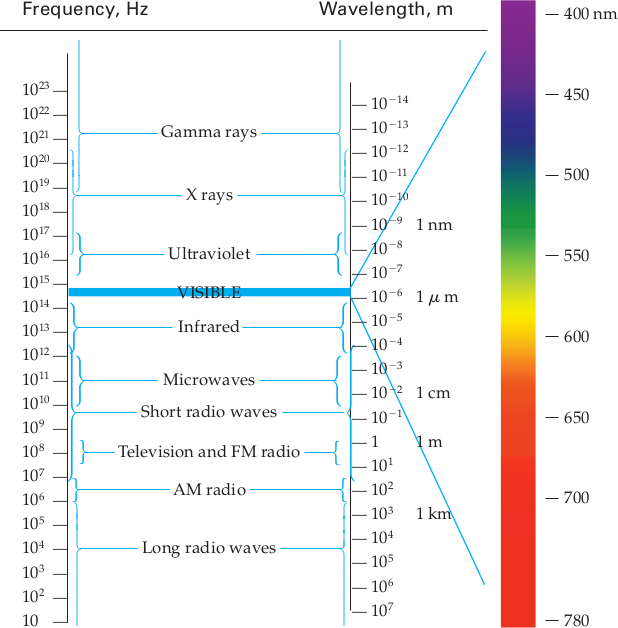
\includegraphics[width=0.8\textwidth]{images/3/31-espectre.png}
\caption{Espectre electromagnètic segons $\nu$ i $\lambda$.}
\end{figure}

\begin{figure}[H]
\centering
    WIP: GRAFIC BONIC 
\caption{Intensitat segons la font de llum}
\end{figure}

\subsubsection*{Dualitat ona--corpuscle}
Els fotons de llum estan quantitzats, de manera que $E$ només pot agafar valors que siguin múltiples enters de:
\begin{align}
    \boxed{E = h \nu = h \frac{v}{\lambda}}
\end{align}

on $h = \SI{6.626 e-34}{\J\s} = \SI{4.136 e-15}{\eV\s}$.

\subsubsection*{Interacció llum--matèria}
\begin{figure}[H]
\centering
    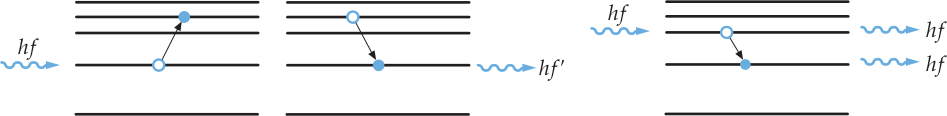
\includegraphics[width=\textwidth]{images/3/31-interaccio.png}
\caption{Processos d'absorció, emissió espontània i emissió estimulada, respectivament}
\end{figure}
\begin{itemize}
    \item Absorció de llum
    \item Emissió de llum
        \subitem Espontània
            \subsubitem Fluorescència: $\tau \sim \SI{10 e-8}{\s}$.
            \subsubitem Fosforescència: $\tau \uparrow \sim \si{\s}, \, \si{\minute}, \dots$
        \subitem Estimulada
\end{itemize}
%----------------------------------------------------------------------------------------
\subsection{Propagació de la llum}
\subsubsection*{Principi de Huygens}
Cada punt en un front d'ona primari actua com a font esfèrica secundària. La superposició d'aquests fronts d'ona secundaris és un nou front d'ona primari.
\begin{figure}[H]
\centering
    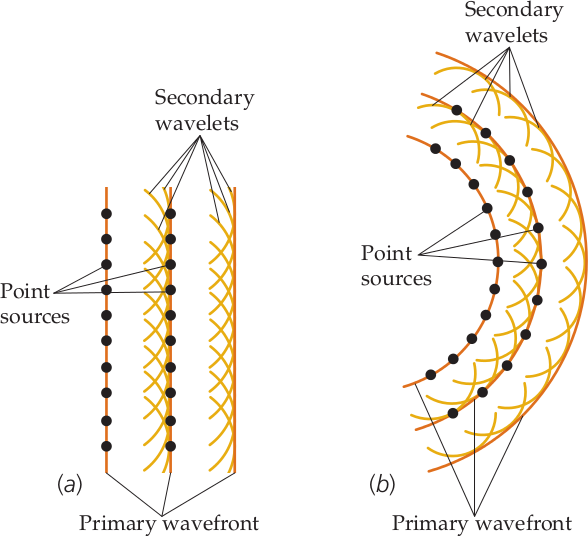
\includegraphics[width=0.6\textwidth]{images/3/32-huygens.png}
\caption{Construcció de Huygens dels fronts d'ona}
\end{figure}

\subsubsection*{Principi de Fermat}
 El camí fet per la llum entre dos punts és tal que el temps de recorregut del qual és mínim.

%----------------------------------------------------------------------------------------
\subsection{Reflexió i refracció}
\begin{figure}[H]
\centering
    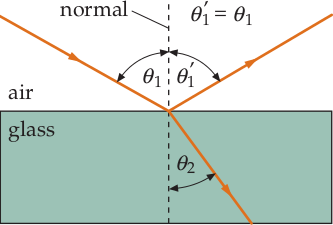
\includegraphics[width=0.5\textwidth]{images/3/33-refl-refr.png}
\caption{Diagrama de reflexió i refracció de la llum quan experimenta un canvi de medi}
\end{figure}
\subsubsection*{Llei de reflexió}
\begin{align}
    \boxed{\theta = \theta '}
\end{align}

\subsubsection*{Llei d'Snell de la refracció}
\begin{align}
    \boxed{n_{1} \sin \theta_{1} = n_{2} \sin \theta_{2}}
\end{align}
on $\begin{gathered} \boxed{n = \frac{c}{v}} \end{gathered}$ és l'índex de refracció de cada medi.

La refracció de la llum és una conseqüència del principi de Fermat.

\subsubsection*{Angle crític de reflexió total}
\begin{figure}[H]
\centering
    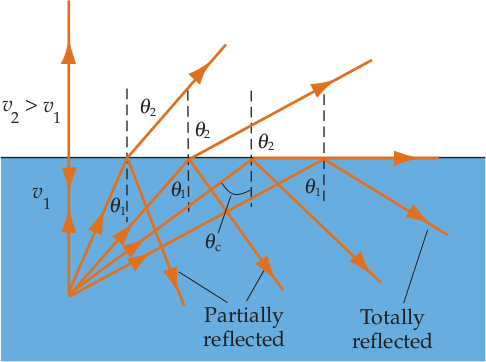
\includegraphics[width=0.6\textwidth]{images/3/33-angle-critic.png}
\caption{Diagrama d l'angle crític de reflexió total interna per a la refracció}
\end{figure}
\begin{align}
    n_{1} \sin \theta_{c} = n_{1} \sin \SI{90}{\degree} \Rightarrow \boxed{\sin \theta_{c} = \frac{n_{2}}{n_{1}}}
\end{align}

\subsubsection*{Casos concrets de refracció}

\subsection{Dispersió}
\subsubsection*{Tipus de superfícies}
\begin{itemize}
    \item Polida: actua com a una superfície especular.
        \begin{figure}[H]
        \centering
            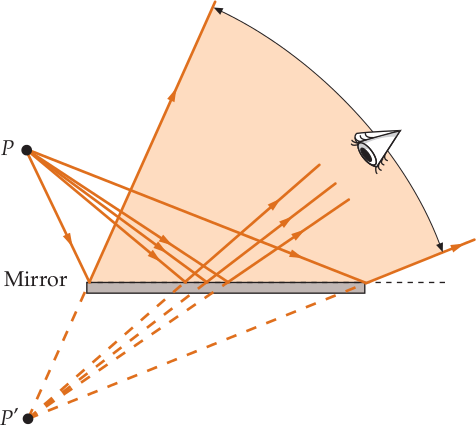
\includegraphics[width=0.4\textwidth]{images/3/34-especular.png}
        \caption{Superfície especular}
        \end{figure}
    \item No polida: actua com a una superfície difusora.
        \begin{figure}[H]
        \centering
            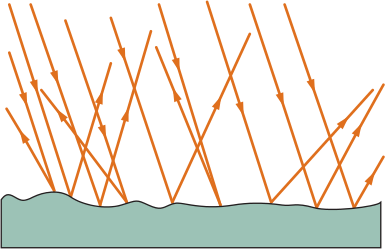
\includegraphics[width=0.4\textwidth]{images/3/34-difusor.png}
        \caption{Superfície difusora}
        \end{figure}
\end{itemize}

\subsubsection*{Dispersió cromàtica}
Com que la freqüència $\nu$ no varia en canviar la llum de medi, $n (\lambda) \Rightarrow$ cada color es refracta en una direcció diferent.
\begin{figure}[H]
\centering
    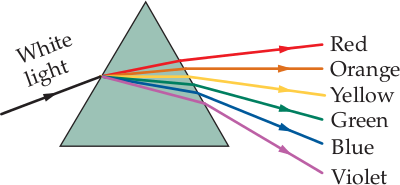
\includegraphics[width=0.6\textwidth]{images/3/34-disp-cromatica.png}
\caption{Dispersió cromàtica de la llum quan passa a través d'un prisma}
\end{figure}

%----------------------------------------------------------------------------------------
\subsection{Polarització de la llum}
En una ona electromagnètica, la direcció del camp elèctric és perpendicular a la direcció de propagació de la ona. Si el camp elèctric roman paral·lel a la direcció de propagació, es diu que l'ona està polaritzada linealment. Les ones produïdes per nombroses fonts no solen estar polaritzades, en aquests casos, el camp elèctric té components $x$ i $y$ que poden variar amb el temps.
\subsubsection*{Dicroisme (absorció selectiva)}

\subsubsection*{Reflexió selectiva}

\subsubsection*{Difusió Rayleigh}

\subsubsection*{Birefringència}
    %----------------------------------------------------------------------------------------
%    ÒPTICA
%----------------------------------------------------------------------------------------
\section{Òptica geomètrica}
\subsection{Miralls plans}
Les imatges formades pels miralls són conseqüència de la reflexió dels rajos de llum que van a parar a ells. Si el que veiem és una imatge formada pròpiament per aquests rajos, es tracta d'una imatge real; si el que veiem és una prolongació dels rajos, es tracta d'una imatge virtual.
\begin{figure}[H]
\centering
    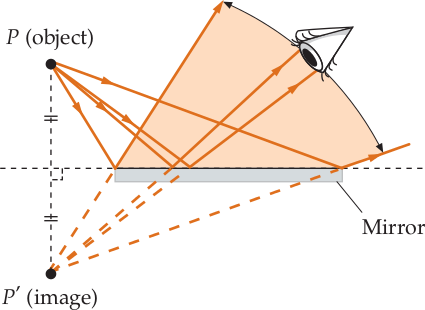
\includegraphics[width=0.5\textwidth]{images/4/41-mirall-pla.png}
\caption{Imatge formada per un mirall pla. Els rajos que venen del punt $P$ que van a parar al mirall sembla que vinguin del punt $P'$; es tracta d'una imatge virtual}
\end{figure}
Si fiques la mà dreta al davant d'un mirall, la imatge no és magnificada ni reduïda, però sembla una mà esquerra. Aquesta reversió dreta--esquerra és el resultat d'una \emph{inversió en profunditat}.

\subsubsection*{Exemples de miralls plans}
\begin{figure}[H]
\centering
    WIP: GRAFIC BONIC 
\caption{Periscopi}
\end{figure}

\begin{figure}[H]
\centering
    WIP: GRAFIC BONIC 
\caption{Caleidoscopi}
\end{figure}

\begin{figure}[H]
\centering
    WIP: GRAFIC BONIC 
\caption{Retroreflector}
\end{figure}

%----------------------------------------------------------------------------------------
\subsection{Miralls esfèrics}
Els miralls còncaus produeixen imatges reals i virtuals, mentre que els miralls convexos només produeixen de virtuals.
\begin{figure}[H]
\centering
    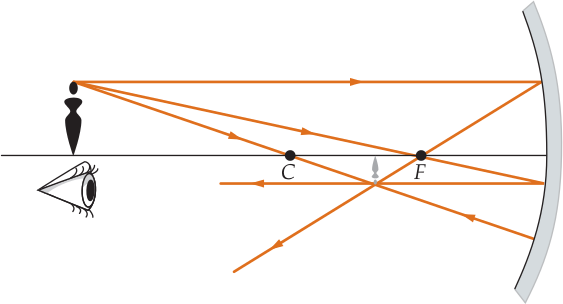
\includegraphics[width=0.6\textwidth]{images/4/42-mirall-esferic.png}
\caption{Imatge formada per un mirall esfèric. Els rajos que venen del punt $P$ que van a parar al mirall convergeixen en el punt $P'$; es tracta d'una imatge real}
\end{figure}

\subsubsection*{Diagrama de rajos per a miralls}
Dels infinits rajos, hi ha tres ---els rajos principals--- que són molt convenients d'emprar:
\begin{enumerate}
    \item Raig paral·lel: dibuixat paral·lel a l'eix. Aquest raig és reflectit al punt focal ($F$).
    \item Raig focal: dibuixat tal que passi pel punt focal ($F$). Aquest raig és reflectit paral·lel a l'eix.
    \item Raig radial: dibuixat tal que passi pel centre de curvatura ($C$). Aquest raig és reflectit en la mateixa direcció de provinença.
\end{enumerate}

La imatge es forma allà on convergeixen aquests tres rajos.

\subsubsection*{Convenció de signes}
\begin{enumerate}
    \item $s$ és positiva si l'objecte està a la banda de la llum incident del mirall.
    \item $s'$ és positiva si la imatge es forma a la banda de la llum reflectida del mirall.
    \item $r$ (i, per tant, $f$) és positiva si el mirall és còncau, de manera que el centre de curvatura està a la banda de la llum reflectida del mirall.
\end{enumerate}
Assumint que tots els rajos són paraxials (aproximadament paral·lels a l'eix), podem establir la següent relació:
\begin{align}
    \boxed{\frac{1}{s} + \frac{1}{s'} = \frac{2}{r}} \label{eq:miralls1}
\end{align}
Es pot establir una relació entre les llargades dels objectes i les seves posicions, que anomenem magnificació lateral de la imatge:
\begin{align}
    \boxed{m = \frac{y'}{y} = - \frac{s'}{s}}
\end{align}
Quan els rajos venen de l'infinit, la imatge es forma al punt focal $F$. La distància entre el mirall i aquest punt s'anomena distància focal i es defineix com a:
\begin{align}
    \boxed{f = \frac{1}{2} r}
\end{align}

Així doncs, podem reescriure l'equació \ref{eq:miralls1}, que anomenem equació dels miralls:
\begin{align}
    \boxed{\frac{1}{s} + \frac{1}{s'} = \frac{1}{f}} \label{eq:miralls2}
\end{align}

%----------------------------------------------------------------------------------------
\subsection{Lents}
\subsubsection*{Imatges formades per refracció}
\begin{figure}[H]
\centering
    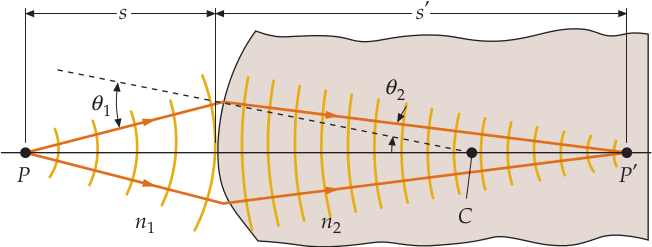
\includegraphics[width=0.8\textwidth]{images/4/43-refraccio.png}
\caption{Imatge formada per la refracció de la llum a una sola superfície esfèrica}
\end{figure}
\begin{align}
    \boxed{\frac{n_{1}}{s} + \frac{n_{2}}{s'} = \frac{n_{2} - n_{1}}{r}}
\end{align}
\subsubsection*{Convenció de signes}
\begin{enumerate}
    \item $s$ és positiva si l'objecte està a la banda de la llum incident de la superfície.
    \item $s'$ és positiva si la imatge es forma a la banda de la llum refractada de la superfície.
    \item $r$ és positiva si el centre de curvatura està a la banda de la llum refractada de la superfície.
\end{enumerate}
La magnificació causada per la refracció a una superfície esfèrica és:
\begin{align}
    \boxed{m = \frac{y'}{y} = - \frac{n_{1} s'}{n_{2} s}}
\end{align}

%----------------------------------------------------------------------------------------
\subsection{Lents primes}
\subsubsection*{Tipus de lents}
\begin{figure}[H]
\centering
    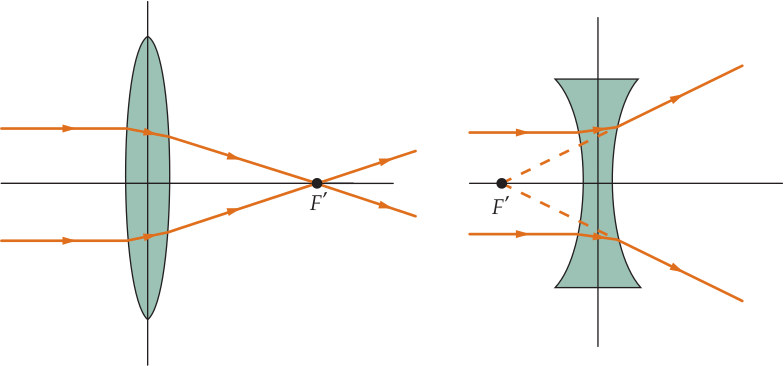
\includegraphics[width=0.9\textwidth]{images/4/44-conv-div.png}
\caption{Lents convergent i divergent, respectivament}
\end{figure}
\begin{figure}[H]
\centering
    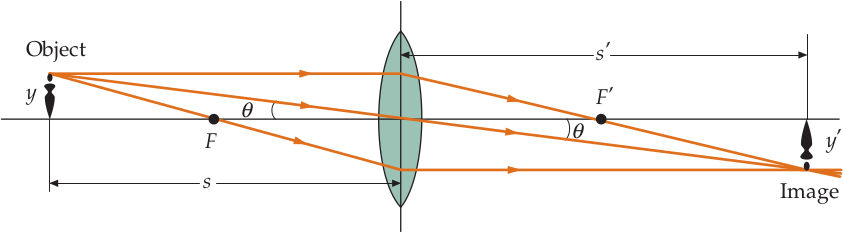
\includegraphics[width=\textwidth]{images/4/44-lents-primes.png}
\caption{Imatge formada per una lent prima convergent. Els rajos que venen del l'objecte van a parar a la lent i convergeixen formant una imatge real}
\end{figure}

\subsubsection*{Diagrama de rajos per a lents}
Dels infinits rajos, hi ha tres ---els rajos principals--- que són molt convenients d'emprar:
\begin{enumerate}
    \item Raig paral·lel: dibuixat paral·lel a l'eix. Aquest raig es dirigeix al segon punt focal de la lent ($F'$).
    \item Raig focal: dibuixat tal que passi pel primer punt focal ($F$). Aquest raig emergeix paral·lel a l'eix.
    \item Raig central: dibuixat tal que passi pel centre de la lent. Aquest raig no canvia la seva direcció\footnote{En realitat, les cares de les lents són paral·leles al centre, de manera que el raig emergeix en la mateixa direcció però desplaçat lleugerament. Com que la lent és prima, aquest fet és negligible.}.
\end{enumerate}
La imatge es forma allà on convergeixen aquests tres rajos.

L'equació creadora de lents és la següent:
\begin{align}
    \boxed{\frac{1}{f} = \left( \frac{n'}{n} - 1 \right) \left( \frac{1}{r_{1}} - \frac{1}{r_{2}} \right)}
\end{align}
L'equació de les lents primes és la mateixa que l'equació dels miralls \eqref{eq:miralls2}:
\begin{align}
    \boxed{\frac{1}{s} + \frac{1}{s'} = \frac{1}{f}}
\end{align}
La magnificació lateral d'una lent és:
\begin{align}
    \boxed{m = \frac{y'}{y} = - \frac{s'}{s}}
\end{align}

\subsubsection*{Potència d'una lent}
El recíproc de la distància focal s'anomena potència d'una lent. Quan la distància focal és expressada en metres, la potència s'expressa en diòptries ($D = \si{\per\m}$).
\begin{align}
    \boxed{P = \frac{1}{f}}
\end{align}

\subsubsection*{Combinació de lents}
Si tenim dues o més lents primes, podem trobar la imatge final produïda pel sistema cercant la distància de la imatge per a la primera lent i després utilitzant-la, juntament amb la distància entre les lents, per trobar la distància de l'objecte de la segona lent. És a dir, considerem cada imatge, si real o virtual ---i si és realment formada o no--- com a objecte per a la següent lent.
\begin{figure}
\centering
    WIP: GRAFIC BONIC 
\caption{Combinació de lents}
\end{figure}

\subsubsection*{Dues lents en contacte}
Quan tenim dues lents en contacte, la distància focal eficient és donada per la següent equació: 
\begin{align}
    \boxed{\frac{1}{f_{ef}} = \frac{1}{f_{1}} + \frac{1}{f_{2}}}
\end{align}
La potència eficient de dues lents en contacte és:
\begin{align}
    \boxed{P_{ef} = P_{1} + P_{2}}
\end{align}

%----------------------------------------------------------------------------------------
\subsection{Aberracions}
Quan tots els rajos des d'un objecte puntual no convergeixen en una única imatge puntual, el desenfocament resultant s'anomena aberració. 
\begin{figure}[H]
\centering
    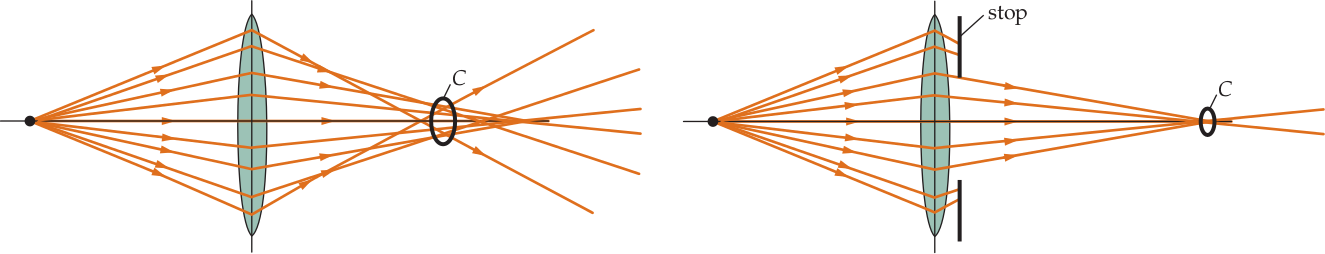
\includegraphics[width=\textwidth]{images/4/45-aberracions.png}
\caption{L'aberració esfèrica produïda per una lent es pot disminuir reduint l'obertura amb un diafragma.}
\end{figure}
    %----------------------------------------------------------------------------------------
%    INSTRUMENTS ÒPTICS
%----------------------------------------------------------------------------------------
\section{Instruments òptics}
\subsection{Ull humà}
\begin{figure}[H]
\centering
    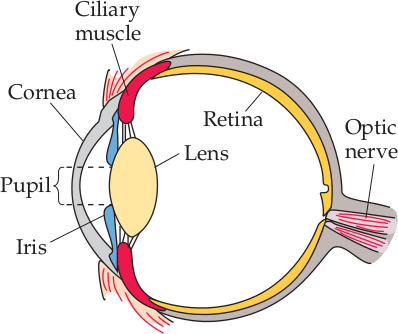
\includegraphics[width=0.5\textwidth]{images/5/51-ull.png}
\caption{Diagrama de l'ull humà}
\end{figure}

\subsubsection*{Característiques òptiques de l'ull}
\begin{itemize}
    \item Pupil·la: Té un diàmetre variable de $\sim \SIrange[range-phrase= -]{2}{8}{\mm}$.
    \item Cristal·lí: $n_{C} \approx \numrange[range-phrase = -]{1.386}{1.406}$ (enfoc variable).
        \subitem Cons: cèl·lules fotosensibles que permeten distingir els colors. N'hi ha $\sim \numrange[range-phrase = -]{6e6}{7e6}$.
        \subitem Bastons: cèl·lules fotosensibles que capten l'intensitat de llum. N'hi ha $\sim 125 \times 10^{6}$.
    \item Còrnia: quan el cristal·lí està relaxat, la distància focal del sistema còrnia--cristal·lí és de $\SI{2.5}{cm}$, que és la distància entre la còrnia i la retina.
    \item Humor aquós i vitri: $n_{A} \approx 1.336$, $n_{V}\approx 1.336$.
    \item Punt proper ($x_{pp}$): és el punt més proper pel qual el cristal·lí pot enfocar la imatge a la retina. S'agafa $\SI{25}{\cm}$ com a valor estàndard.
\end{itemize}

\subsubsection*{Defectes de l'ull}
\begin{itemize}
    \item Miopia: la imatge es forma abans de la retina. S'arregla amb lents divergents.
    \item Hipermetropia: la imatge es forma després de la retina. S'arregla amb lents convergents.
    \item Presbícia: la distància més propera disminueix.
\end{itemize}

\subsubsection*{Mida aparent d'un objecte}
\begin{figure}[H]
\centering
    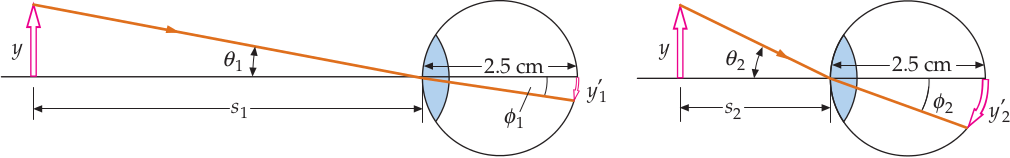
\includegraphics[width=\textwidth]{images/5/51-ull-imatge.png}
\caption{Diagrama de formació d'imatges sobre la retina de l'ull. Un objecte llunyà sembla petit perquè la seva imatge és més petita que la del mateix objecte més proper a l'ull}
\end{figure}
\begin{align}
    \boxed{\phi = \frac{y'}{\SI{2.5}{\cm}}} \quad \boxed{\theta \approx \frac{y}{s}}
\end{align}
Aplicant la llei d'Snell per a la refracció, tenim que $n_{aire} \sin \theta = n \sin \phi$, on $n$ és l'índex de refracció de l'interior de l'ull. Llavors, per a angles petits:
\begin{align}
    \boxed{\theta \approx n \phi}
\end{align}
Així doncs, combinant les equacions anteriors, tenim:
\begin{align}
    \boxed{y' = \frac{\SI{2.5}{\cm}}{n} \frac{y}{s}}, \quad s \geq x_{pp} = \SI{25}{\cm}
\end{align}

%----------------------------------------------------------------------------------------
\subsection{Magnificador simple}
Una lent convergent s'anomena magnificador simple o lupa si se situa a prop de l'ull i si l'objecte se situa de la lent a una distància inferior a la seva distància focal.
\begin{figure}[H]
\centering
    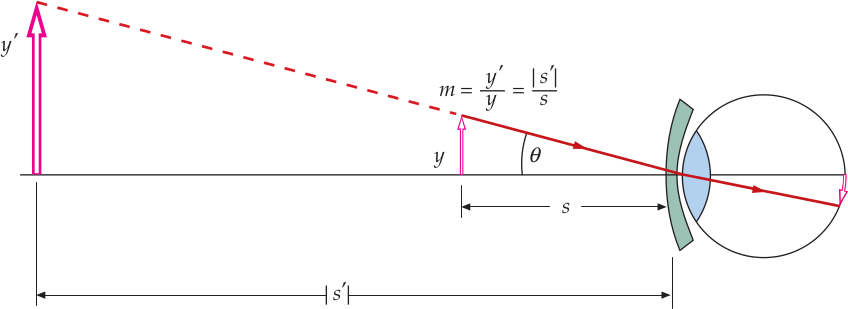
\includegraphics[width=\textwidth]{images/5/52-magnificador.png}
\caption{Diagrama de rajos d'un magnificador simple}
\end{figure}
Per a l'ull, la imatge d'un objecte subtendeix un angle $\theta$ donat per aproximadament:
\begin{align}
    \boxed{\theta \approx \frac{y}{s} = \frac{y'}{|s'|}}
\end{align}
\subsubsection*{Poder magnificador}
L'angle màxim que pot subtendir l'ull és $\begin{gathered}\theta_{o} = \frac{y}{x_{pp}}\end{gathered}$ (amb l'objecte al punt proper), però quan posem al davant un magnificador simple, aquest angle màxim augmenta fins a $\begin{gathered}\theta = \frac{y}{f}\end{gathered}$ (posant l'objecte a la distància focal). 

Llavors, definim el poder magnificador o amplificació angular d'una lent com a:
\begin{align}
    \boxed{M = \frac{\theta}{\theta_{o}} = \frac{x_{pp}}{f}}
\end{align}
Aleshores, un magnificador simple permet enfocar objectes a una distància molt propera (de manera que la seva imatge formada a la retina és major) amb l'ull relaxat.

%----------------------------------------------------------------------------------------
\subsection{Microscopi compost}
\begin{figure}[H]
\centering
    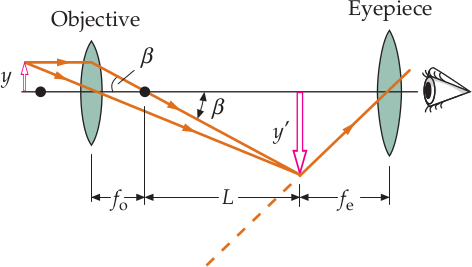
\includegraphics[width=0.6\textwidth]{images/5/53-microscopi.png}
\caption{Diagrama de rajos d'un microscopi òptic compost. Està composat per, d'esquerra a dreta un objectiu i un ocular}
\end{figure}
La magnificació lateral $m_{o}$ de l'objectiu és:
\begin{align}
    \boxed{m_{o} = \frac{y'}{y} = - \frac{L}{f_{o}}}
\end{align}
on $f_{o}$ és la distància focal de l'objectiu i $L$ és la distància entre la focal de l'objectiu i la focal de l'ocular; l'anomenem distància del tub.

El poder magnificador de l'ocular és:
\begin{align}
    \boxed{M_{e} = \frac{x_{pp}}{f_{e}}}
\end{align}
El poder magnificador del sistema compost és el producte dels augments de l'objectiu i l'ocular:
\begin{align}
    \boxed{M = m_{o} M_{e} = - \frac{L}{f_{o}} \frac{x_{pp}}{f_{e}}}
\end{align}

\subsubsection*{Valors estàndard dels augments}
\begin{itemize}
    \item $m_{o}$: $4 \times$, $10 \times$, $20 \times$, $40 \times$, $100 \times$.
    \item $M_{e}$: $10 \times$, $20 \times$.
\end{itemize}

%----------------------------------------------------------------------------------------
\subsection{Telescopi}
\begin{figure}[H]
\centering
    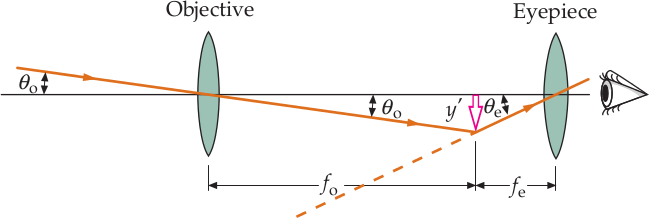
\includegraphics[width=0.8\textwidth]{images/5/54-telescopi.png}
\caption{Diagrama de rajos d'un telescopi}
\end{figure}
Podem fer les aproximacions per a angles petits següents:
\begin{align}
    \boxed{\tan \theta_{o} = \frac{y}{s} = - \frac{y'}{f_{o}} \approx \theta_{o}}
\end{align}
\begin{align}
    \boxed{\tan \theta_{e} = \frac{y'}{f_{e}} \approx \theta_{e}}
\end{align}
com que $y'$ és negativa, $\theta_{e}$ és negativa, indicant que la imatge és invertida.

El poder de magnificació del telescopi és, llavors:
\begin{align}
    \boxed{M = \frac{\theta_{e}}{\theta_{o}} = \frac{f_{o}}{f_{e}}}
\end{align}

\subsubsection*{Telescopi reflector}
\begin{figure}[H]
\centering
    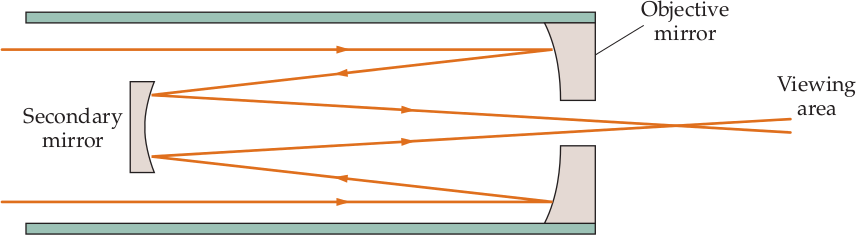
\includegraphics[width=0.9\textwidth]{images/5/54-telescopi-reflector.png}
\caption{Diagrama de rajos d'un telescopi reflector }
\end{figure}
Un telescopi reflector utilitza miralls còncaus en comptes de lents per a l'objectiu. El fet d'utilitzar un mirall té molts avantatges, com ara eliminar la aberració cromàtica.

\subsubsection*{Telescopi de Galileu}
WIP: stuff.
    %----------------------------------------------------------------------------------------
%    INTERFÈNCIA I DIFRACCIÓ
%----------------------------------------------------------------------------------------
\section{Interferència i difracció}
\subsection{Diferència de fase i coherència}
Quan dues ones harmòniques de la mateixa freqüència i longitud se superposen, tenim:
\begin{align}
    \boxed{I_{T} = I_{1} + I_{2} + 2 \sqrt{I_{1} I_{2}} \cos \delta}
\end{align}

i $\delta$, la diferència de fase deguda a una diferència de camins, ve donada per:
\begin{align}
    \boxed{\delta = k \Delta r = \frac{2 \pi}{\lambda} \Delta r}
\end{align}
Si $\delta = 2 \pi m$, tenim una interferència constructiva. En canvi, si és $\delta = (2m-1) \pi$, és destructiva. ($m \in \mathbb{N}$).

Quan una ona és reflectida en una superfície d'un medi pel qual viatja més lentament, es produeix un canvi de fase de la llum reflectida de $\boxed{\delta_{R} = \pi}$.

%----------------------------------------------------------------------------------------
\subsection{Interferència en làmines primes}
\begin{figure}[H]
\centering
    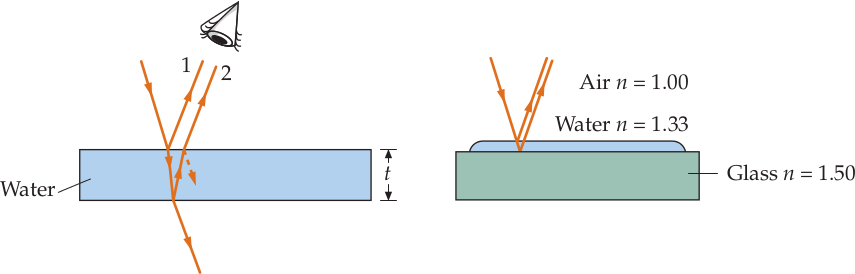
\includegraphics[width=0.9\textwidth]{images/6/62-lamines.png}
\caption{Diagrama de rajos que impacten en làmines primes}
\end{figure}
A més de la diferència de fase produïda per la diferència de camins $\delta = 4t \pi / \lambda$, s'ha de tenir en compte la diferència de fase $\delta_{R}$ produïda en la reflexió sobre una superfície de $n' > n$.

\begin{figure}[H]
\centering
    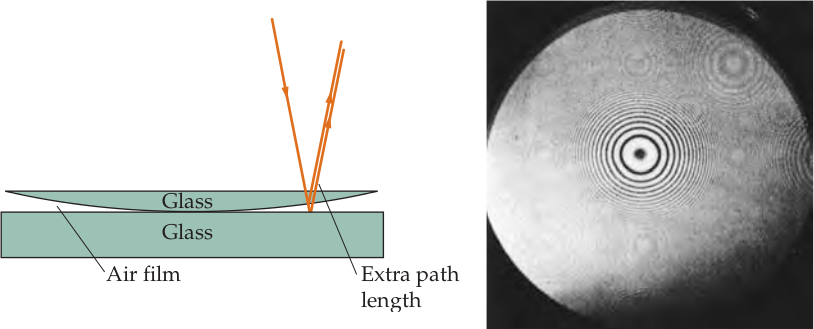
\includegraphics[width=0.9\textwidth]{images/6/62-newton.png}
\caption{Diagrama del muntatge dels anells de Newton. Es forma un anell quan augmentem el gruix de l'aire en $\pi$}
\end{figure}
\begin{figure}[H]
\centering
    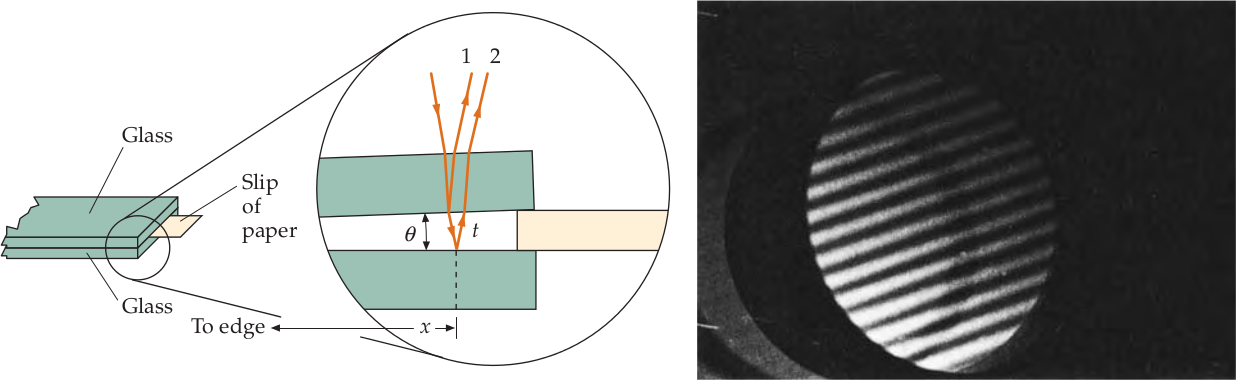
\includegraphics[width=\textwidth]{images/6/62-fizeau.png}
\caption{Diagrama del muntatge de les franges de Fizeau, que són equidistants}
\end{figure}

\subsubsection*{Pel·lícules anti-reflectants}
Són pel·lícules que per a certes longituds d'ona, la superposició d'ones harmòniques és destructiva, de manera que a fins pràctis no reflecteix. Les pel·lícules acostumen a tenir un índex de refracció de $n = 1.38$.

%----------------------------------------------------------------------------------------
\subsection{Divisió d'amplitud}
Un exemple és l'interferòmetre de Michelson.

%----------------------------------------------------------------------------------------
\subsection{Divisió de fronts d'ona}
\begin{figure}[H]
\centering
    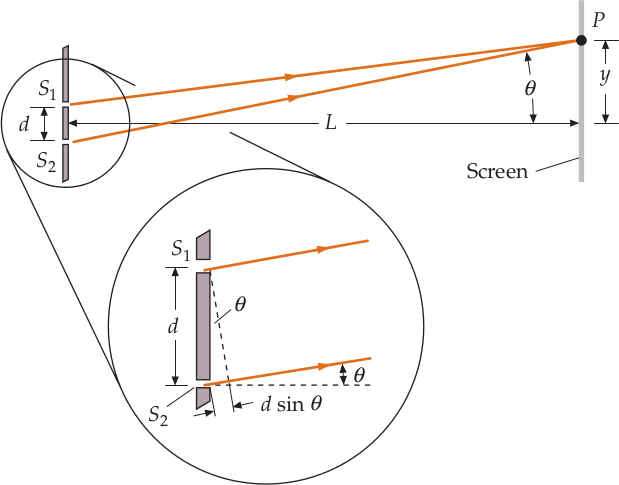
\includegraphics[width=0.6\textwidth]{images/6/64-int-doble.png}
\caption{Diagrama de la doble escletxa de Young}
\end{figure}
\subsubsection*{Patró d'interferència de dues escletxes}
\begin{itemize}
    \item Màxims: $\begin{gathered} \boxed{d \sin \theta_{m} = m \lambda} \end{gathered}, \quad m = 0, 1, 2 \dots$
    \item Mínims: $\begin{gathered} \boxed{d \sin \theta_{m} = (m - \frac{1}{2}) \lambda} \end{gathered}, \quad m = 1, 2, 3 \dots$
\end{itemize}
on $m$ és l'ordre d'interferència.

La diferència de fase ve donada per:
\begin{align} 
    \delta = d \sin \theta \frac{2 \pi}{\lambda} 
\end{align}
Podem relacionar la distància de les escletxes $L$ a la pantalla amb la distància $y_{m}$ a través de la pantalla:
\begin{align}
    \tan \theta_{m} = \frac{y_{m}}{L}
\end{align}
Llavors, per a angles petits $\tan \theta \approx \sin \theta$, i podem deduir:
\begin{align}
    \boxed{y_{m} = m \frac{\lambda L}{d}}
\end{align}

\subsubsection*{Càlcul de la intensitat}
\begin{align}
    \boxed{I = 4 I_{0} \cos^2 \left( \frac{1}{2} \delta \right)}
\end{align}

on $I_{0}$ és la intensitat de llum que arriba de cada escletxa i $\delta$ està relacionada amb la la posició a la pantalla.

%----------------------------------------------------------------------------------------
\subsection{Difracció}
\subsubsection*{Patró de difracció d'una escletxa}
\begin{figure}[H]
\centering
    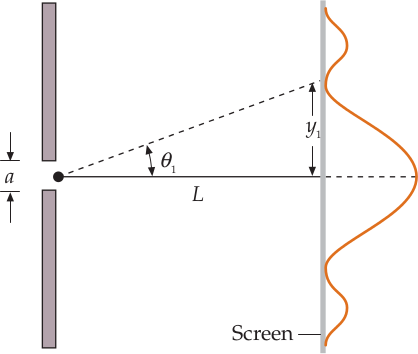
\includegraphics[width=0.4\textwidth]{images/6/65-dif-una.png}
\caption{Diagrama de difracció causada per una escletxa}
\end{figure}
\begin{itemize}
    \item Punts d'intensitat $I=0$: $\begin{gathered} \boxed{a \sin \theta_{m} = m \lambda} \end{gathered}, \quad m = 1, 2, 3 \dots$
\end{itemize}
Podem relacionar la distància de les escletxes $L$ a la pantalla amb la distància $y_{m}$ a través de la pantalla:
\begin{align}
    \tan \theta_{m} = \frac{y_{m}}{L}
\end{align}
Llavors, per a angles petits $\tan \theta \approx \sin \theta$, i podem deduir els punts d'intensitat zero:
\begin{align}
    \boxed{y_{m} = m \frac{\lambda L}{a}}
\end{align}

\subsubsection*{Patró d'interferència--difracció de dues escletxes}
\begin{figure}[H]
\centering
    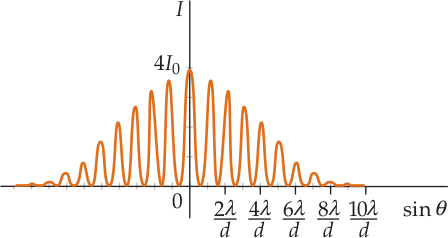
\includegraphics[width=0.6\textwidth]{images/6/65-int-dif-doble.png}
\caption{Diagrama de difracció causada per una escletxa}
\end{figure}
Al màxim central d'intensitat per difracció hi ha $N$ pics d'intensitat màxima per interferència. Com que el $m$-èsim màxim d'interferència és d'intensitat zero per difracció, tenim $m-1$ pics a cada banda del pic central. Llavors:
\begin{align}
    \boxed{N = 2(m-1) + 1 = 2m - 1}
\end{align}
Llavors, $m$ és l'ordre d'interferència tal que el primer mínim de difracció sigui igual a l'$m$-èsim màxim d'interferència:
\begin{align}
\begin{gathered}
    \sin \theta_{1} = \frac{\lambda}{a} = \sin \theta_{m} = m \frac{\lambda}{d}\\
    \Rightarrow \boxed{m = \frac{d}{a}} \Rightarrow \boxed{N = 2 \frac{d}{a} - 1}    
\end{gathered}
\end{align}

%----------------------------------------------------------------------------------------
\subsection{Ús de fasors per sumar ones harmòniques}
\subsubsection*{Patró d'interferència de tres o més fonts separades per la mateixa distància}
\subsubsection*{Patró d'interferència--difracció de múltiples escletxes}
\subsubsection*{Xarxa de difracció}

%----------------------------------------------------------------------------------------
\subsection{Difracció de Fraunhofer i Fresnel}
\begin{figure}[H]
\centering
    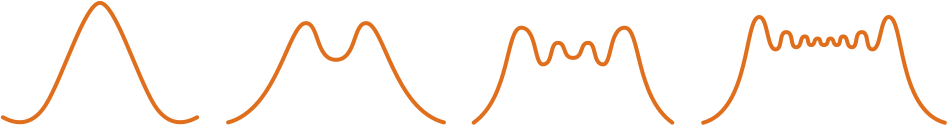
\includegraphics[width=\textwidth]{images/6/65-fraunhofer-fresnel.png}
\caption{El patró de difracció de Fraunhofer (paraxial) canvia gradualment al de difracció de Fresnel (no paraxial) quan apropem l'objecte a l'escletxa}
\end{figure}

\subsubsection*{Difracció i resolució}
La difracció a casa d'una obertura circular té importants implicacions per a la resolució de diferents instruments òptics. L'angle $\theta$ subtendit pel primer mínim difracció de Fraunhofer està relacionat amb la longitud d'ona i el diàmetre $D$ de l'obertura:
\begin{align}
    \boxed{\sin \theta = 1.22 \frac{\lambda}{D}}
\end{align}
En moltes aplicacions, l'angle $\theta$ és petit, llavors:
\begin{align}
    \theta \approx 1.22 \frac{\lambda}{D}
\end{align}
Dos focus puntuals subtendeixen un angle $\alpha$ amb l'obertura. Si $\alpha$ és molt major a $1.22 \lambda / D$ es veuran dos focus a l patró de difracció. Llavors per a una separació angular crítica $\alpha_{c}$ els dos focus se solaparan:
\begin{align}
    \boxed{\alpha_{c} = 1.22 \frac{\lambda}{D}}
\end{align}

%----------------------------------------------------------------------------------------
\end{document}